\documentclass[10pt,aspectratio=43,mathserif,table]{beamer} 
%  设置为 Beamer 文档类型,设置字体为 10pt,长宽比为16:9,数学字体为 serif 风格
\batchmode
\usepackage{graphicx}
\usepackage{subfigure}
\usepackage{fontspec}

% \setmainfont{Harding Text Web Regular Regular.ttf}
\usepackage{diagbox} % 表头斜线分区
\usepackage{unicode-math}
\usefonttheme{serif}
% \setmathrm{Harding Text Web Regular Regular.ttf} % 设置数学字体为 Times New Roman
\setmathfont{TeX Gyre Termes Math} % 如果您使用 XeLaTeX 或 LuaLaTeX 编译,可以使用其他数学字体
\setmathtt{Courier New} % 设置等宽字体为 Courier New
\setboldmathrm{Times New Roman}
\setmathfont{TeX Gyre Termes Math}[version=bold] % 设置粗体数学字体
\setmathfont{TeX Gyre Termes Math}[range={\mathit}]


\usetheme{Berlin} %主题
\setbeamertemplate{page number in head/foot}[pagenumber]
%\usecolortheme{sustech} %主题颜色

\usepackage[ruled,linesnumbered]{algorithm2e}

\usepackage{fancybox}
\usepackage{xcolor}
\usepackage{listings}

\usepackage{booktabs}
\usepackage{colortbl}

\newcommand{\Console}{Console}
\lstset{ %
	backgroundcolor=\color{white},   % choose the background color
	basicstyle=\footnotesize\rmfamily,     % size of fonts used for the code
	columns=fullflexible,
	breaklines=true,                 % automatic line breaking only at whitespace
	captionpos=b,                    % sets the caption-position to bottom
	tabsize=4,
	commentstyle=\color{mygreen},    % comment style
	escapeinside={\%*}{*)},          % if you want to add LaTeX within your code
	keywordstyle=\color{blue},       % keyword style
	stringstyle=\color{mymauve}\ttfamily,     % string literal style
	numbers=left, 
	%	frame=single,
	rulesepcolor=\color{red!20!green!20!blue!20},
	% identifierstyle=\color{red},
	language=c
}


\definecolor{mygreen}{rgb}{0,0.6,0}
\definecolor{mymauve}{rgb}{0.58,0,0.82}
\definecolor{mygray}{gray}{.9}
\definecolor{mypink}{rgb}{.99,.91,.95}
\definecolor{mycyan}{cmyk}{.3,0,0,0}

%题目,作者,学校,日期
\title{Paper Reading}
%\subtitle{\fontsize{9pt}{14pt}\textbf{跨临界分岔}}
\author{Speaker: Yichen Lu\quad \newline  \newline \quad }
\institute{\fontsize{8pt}{14pt}}
\date{\today}
\newcommand{\concept}{Paper Reading}

%学校Logo
%\pgfdeclareimage[height=0.5cm]{sustech-logo}{sustech-logo.pdf}
%\logo{\pgfuseimage{sustech-logo}\hspace*{0.3cm}}

\AtBeginSection[]
{
	\begin{frame}<beamer>
	\frametitle{\textbf{Contents}}
	\tableofcontents[currentsection]
\end{frame}
}
% \beamerdefaultoverlayspecification{<+->}
% -----------------------------------------------------------------------------
\begin{document}
% -----------------------------------------------------------------------------
% \frame{\titlepage}

% \frame{\titlepage}
\begin{frame}
    \begin{figure}
        \centering
        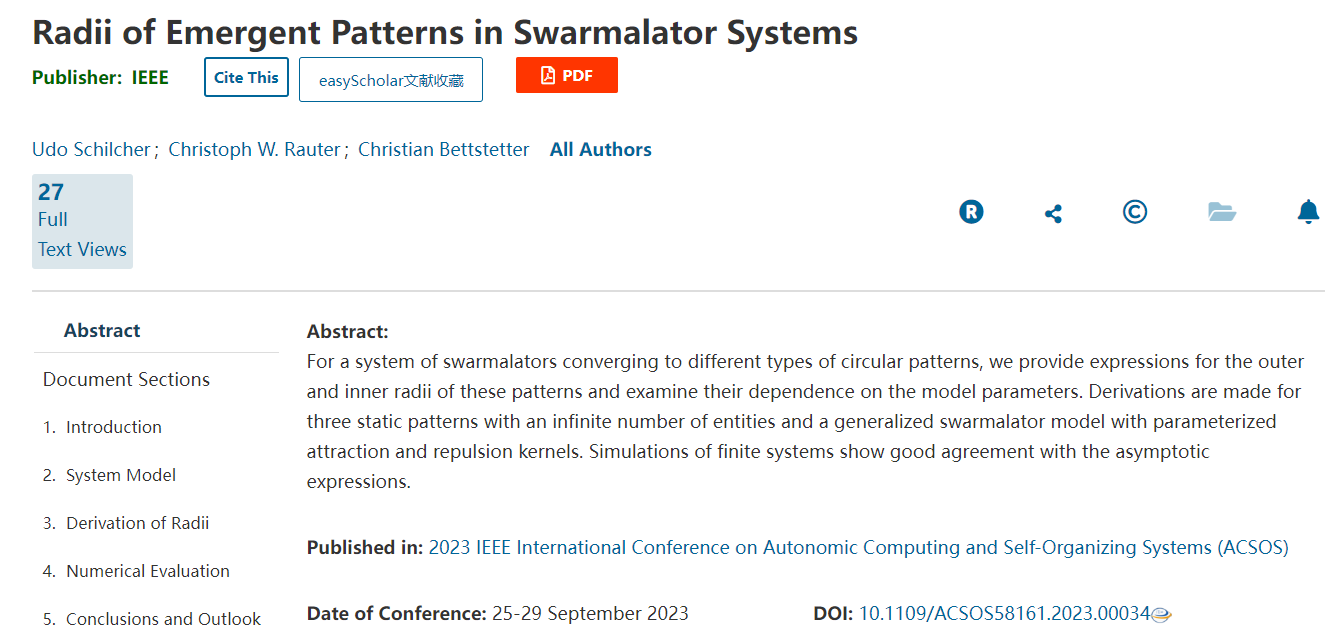
\includegraphics[width=\textwidth]{front.jpg}
    \end{figure}
\end{frame}


\begin{frame}
    Model equations:
    $$
    \begin{aligned}
        \dot{\boldsymbol{x}}_i&=\frac{1}{N}\sum_{j\ne i}^N{e_{ij}d_{ij}^{\alpha}\left( 1+J\cos \theta _{ij} \right) -e_{ij}d_{ij}^{\beta}}\\
        \dot{\theta}_i&=\frac{K}{N}\sum_{j\ne i}^N{d_{ij}^{\gamma}\sin \theta _{ij}}\\
    \end{aligned}
    $$
    where 
    $d_{ij}=\left\| \boldsymbol{x}_j-\boldsymbol{x}_i \right\|$, 
    $\theta _{ij}=\theta _i-\theta _j$, 
    $e_{ij}=\cfrac{1}{d_{ij}}(\boldsymbol{x}_j-\boldsymbol{x}_i)$.

    Choosing $\alpha = 0$ and $\beta=\gamma=-1$ gives the original model.
\end{frame}

\begin{frame}
    In the converged state of the static patterns, the entities no longer move, so we have $\dot{\boldsymbol{x}}_i = 0$, which yields:

    $$
    r_{\mathrm{out}}^{\alpha}\underset{\mathrm{Attraction} A}{\underbrace{\sum_{j\ne i}^N{e_{ij}g_{ij}^{\alpha}\left( 1+J\cos \theta _{ij} \right)}}}=r_{\mathrm{out}}^{\beta}\underset{\mathrm{Repulsion} R}{\underbrace{\sum_{j\ne i}^N{e_{ij}g_{ij}^{\alpha}}}}
    $$

    where $r_{\mathrm{out}}=\underset{1\le i\le N}{\max}\left\| \boldsymbol{x}_i-\bar{\boldsymbol{x}} \right\| $, 
    $g_{ij}=\frac{d_{ij}}{r_{\mathrm{out}}}$.



\end{frame}






% -----------------------------------------------------------------------------
\end{document}